% Independent manuscript derived from framework.png and framework_locomo_example.png.
% Empirical evaluation is planned, not completed. Never replace missing results with guesses.
\documentclass{article}
\usepackage{iclr2027_conference,times}
\usepackage[T1]{fontenc}
\usepackage{amsmath,amssymb,booktabs,tabularx,graphicx,hyperref,url}
\usepackage{algorithm,algpseudocode,placeins,etoolbox}
\hypersetup{colorlinks=true,linkcolor=blue,citecolor=blue,urlcolor=blue}
\newcommand{\method}{MTM}
\newcommand{\E}{\mathcal{E}}
\newcommand{\Sema}{\mathcal{S}}
\newcommand{\Proc}{\mathcal{P}}
\newcommand{\Graph}{\mathcal{G}}
\newcommand{\Queue}{\mathcal{Q}}
\newcommand{\ind}{\mathbf{1}}
\title{Brain-Inspired Multi-Timescale Memory\\for Language Agents}
\author{Anonymous authors}
% Working-copy presentation only. The official style files are unmodified.
\makeatletter
\patchcmd{\@maketitle}{Paper under double-blind review}{Manuscript in preparation}{}{}
\makeatother
\begin{document}
\maketitle
\lhead{Working manuscript: empirical evaluation pending}

\begin{abstract}
Long-lived language agents must remember not only what was mentioned, but who
experienced it, when it was true, and how it should guide a later decision.
Retrieving a relevant memory does not ensure that these distinctions survive
abstraction, and revising an individual fact does not ensure that its derived
knowledge is revised with it. We propose Multi-Timescale Memory (\method), a
brain-inspired framework that separates rapid episodic encoding, query-time
evidence binding, and slower semantic and procedural consolidation. Its central
mechanism is evidence-bound reconsolidation: each derived memory and each use
of that memory retain explicit dependencies, so a supported correction can
invalidate and rebuild affected knowledge without rewriting unrelated history.
A typed router assembles episodic evidence, semantic claims, and applicable
procedures into a bounded working context; conflict-aware fusion preserves
temporal scope and unresolved uncertainty. We ground the design in a verified
LoCoMo example and specify a compact evaluation on LoCoMo and LongMemEval of
accuracy and cost, component contributions, and update-aware reasoning. The framework and algorithm
are proposed here; benchmark performance and superiority over prior systems
remain to be established experimentally.
\end{abstract}

\section{Introduction}
An agent can remember every important noun and still fail to remember an event.
In a LoCoMo conversation, Caroline recommends \emph{Becoming Nicole} in July.
Three months later, Melanie says that she has been reading ``that book''
recommended earlier. Answering which book Melanie read requires binding the
recommendation, its participants, and the later reading event. A list of book
titles is insufficient; an isolated summary of the later session is also
insufficient. The required memory is a relationship across episodes, grounded
in their sources rather than reconstructed from plausible associations.

This difficulty extends beyond retrieval. Once the agent converts experiences
into a general claim or a reusable procedure, later evidence may change the
conditions under which that abstraction is valid. Correcting a source fact
without revisiting its dependent summaries can leave stale knowledge active.
Conversely, replacing all old information with the latest statement destroys
historical distinctions. Useful memory therefore requires coordinated
\emph{encoding, binding, abstraction, and revision}, not simply a larger store.

Existing research already addresses important parts of this problem. Associative
retrieval connects distant evidence; temporal graphs represent evolving facts;
agentic notes revise linked memories; and sleep-time updates reduce online
maintenance overhead \citep{mrw_hipporag,mrw_zep,mrw_amem,mrw_lightmem}.
Reflection and memory-utility learning also make feedback part of memory
management \citep{mrw_reflexion,mrw_hindsight,mrw_memrl}. We do not claim that
these systems lack structure, temporal reasoning, or feedback. The question
we isolate is more specific: \emph{can the path from source experience to
abstraction to use also serve as the path along which a correction propagates?}

Our framework draws a functional analogy to complementary memory processes.
Rapid encoding preserves individual experiences, while slower integration
constructs reusable knowledge \citep{brain_cls1995,brain_cls2016}. Retrieval
brings relevant information into an active context, and subsequent revision
can be restricted to the reactivated knowledge. This is an engineering
interpretation, not an anatomical model or a claim that an LLM reproduces human
cognition. Brain-inspired staging alone is not a new contribution: HippoRAG
and LightMem explicitly adopt related motivations.

\method{} instantiates the analogy with three long-term memory types and
three update timescales. Episodic memory stores observations; semantic memory
stores source-backed claims; procedural memory stores conditional retrieval
or action strategies. A shared dependency graph binds these representations.
At inference time, the agent retrieves and checks evidence before answering.
At revision time, observable corrections identify a dependency-local repair
set. At background consolidation time, replay rebuilds affected abstractions
and validates reusable procedures. An answer generated by the agent is never,
by itself, evidence that the answer is correct.

The intended contribution is a concrete \emph{evidence-bound reconsolidation}
algorithm, rather than a collection of brain-named modules. We specify its
record types, routing rule, conflict semantics, update boundaries, and failure
behavior. A source-verified case illustrates why relational binding matters.
The evaluation uses two conversational benchmarks to test overall utility at
a common budget, isolate component contributions, and examine relational and
update-aware reasoning. The empirical claims remain open until these tests
are run.

% Adapted from ../related_work_20260903.tex. All 38 original citations are retained.
% The former evaluation-study positioning is replaced by this method's positioning.
\section{Related Work}
\label{sec:related_work}

\paragraph{Foundations of agent memory.}
RAG complements parametric knowledge with an external corpus~\citep{mrw_rag}. Early agent systems extend external memory to interaction histories through experience streams and summaries~\citep{mrw_generative_agents,mrw_memorybank}, explicit context hierarchies~\citep{mrw_memgpt}, verbal feedback~\citep{mrw_reflexion}, and reusable executable skills~\citep{mrw_voyager}. These approaches establish complementary forms of persistent state: factual records, compressed context, and experience that can guide subsequent decisions.

\paragraph{Representation, maintenance, and efficient access.}
Later systems organize memory as linked notes or extracted facts~\citep{mrw_amem,mrw_mem0}, associative and temporal graphs~\citep{mrw_hipporag,mrw_hipporag2,mrw_zep,mrw_magma}, and hierarchical or heterogeneous stores~\citep{mrw_memtree,mrw_memoryos,mrw_memos}. Hindsight further distinguishes evidence from synthesized summaries and beliefs~\citep{mrw_hindsight}. Efficiency-oriented approaches combine compression, selective access, and consolidation~\citep{mrw_readagent,mrw_lightmem,mrw_simplemem}; recent systems additionally adapt memory types and structure selection to query requirements~\citep{mrw_leanmem,mrw_mesa}. Their differences concern both how evidence is represented and when computational work is performed. Our question is whether dependencies established across these stages can support targeted revision after new evidence arrives.

\paragraph{Learned policies and execution-time adaptation.}
MEM1, MemAgent, and Memory-R1 learn memory updates or utilization policies through reinforcement learning~\citep{mrw_mem1,mrw_memagent,mrw_memory_r1}. MemRL instead learns the utility of episodic memories without updating model weights~\citep{mrw_memrl}, while MemGen generates latent memory conditioned on the reasoning state~\citep{mrw_memgen}. AdaMEM synthesizes strategies from retrieved trajectories during execution~\citep{mrw_adamem}, and MAGE maintains revisable execution-state trees~\citep{mrw_execution_state}. These approaches already connect memory to decision-making. We distinguish a procedure's applicability and evidence dependencies from its observed usefulness; neither a high retrieval score nor a successful answer establishes that its factual premises remain valid.

\paragraph{Evaluation and unified analyses.}
Conversational benchmarks test long-term recall, reasoning, updates, and reflective memory~\citep{mrw_locomo,mrw_longmemeval,mrw_membench}; incremental interaction and implicit-constraint benchmarks broaden the assessed capabilities~\citep{mrw_memoryagentbench,mrw_locomo_plus}. MemoryArena evaluates memory-dependent multi-session execution, whereas AMA-Bench evaluates understanding of long agent-environment trajectories~\citep{mrw_memoryarena,mrw_amabench}. These settings require distinguishing answer correctness from evidence recovery and successful action. Surveys systematize memory designs and evaluation protocols~\citep{mrw_survey2024,mrw_survey}, and Wu et al. already provide a modular framework and unified empirical comparison~\citep{mrw_memoryeab}. We build on these distinctions, but propose a memory mechanism rather than claim novelty for unified evaluation itself.

\paragraph{Closest overlap and the remaining hypothesis.}
Human-memory-inspired staging is already explicit in LightMem, and associative
binding is central to HippoRAG. Hindsight regenerates synthesized observations
when underlying facts change; A-MEM evolves linked representations. TierMem
uses source-linked retrieval and verified write-back~\citep{brain_tiermem},
while TrustMem verifies memory transitions and learns better update
behavior~\citep{brain_trustmem}. Continuous consolidation can also degrade
useful memory~\citep{brain_faulty}. Consequently, typed storage, source access,
feedback, and selective updates are not individually new. The proposed
distinction is their coupling through \emph{versioned dependencies across
episodic evidence, semantic claims, procedural conditions, and actual use
traces}, with fast invalidation followed by bounded background repair. Its
benefit over these strong alternatives is a hypothesis requiring a matched
comparison, not an established first-of-its-kind claim.


\section{Multi-Timescale Memory}
\label{sec:method}
Figure~\ref{fig:framework} summarizes the framework: fast encoding preserves
episodes, query-time binding constructs a working context, and slower replay
integrates or revises source-backed knowledge.
\begin{figure}[!ht]
\centering
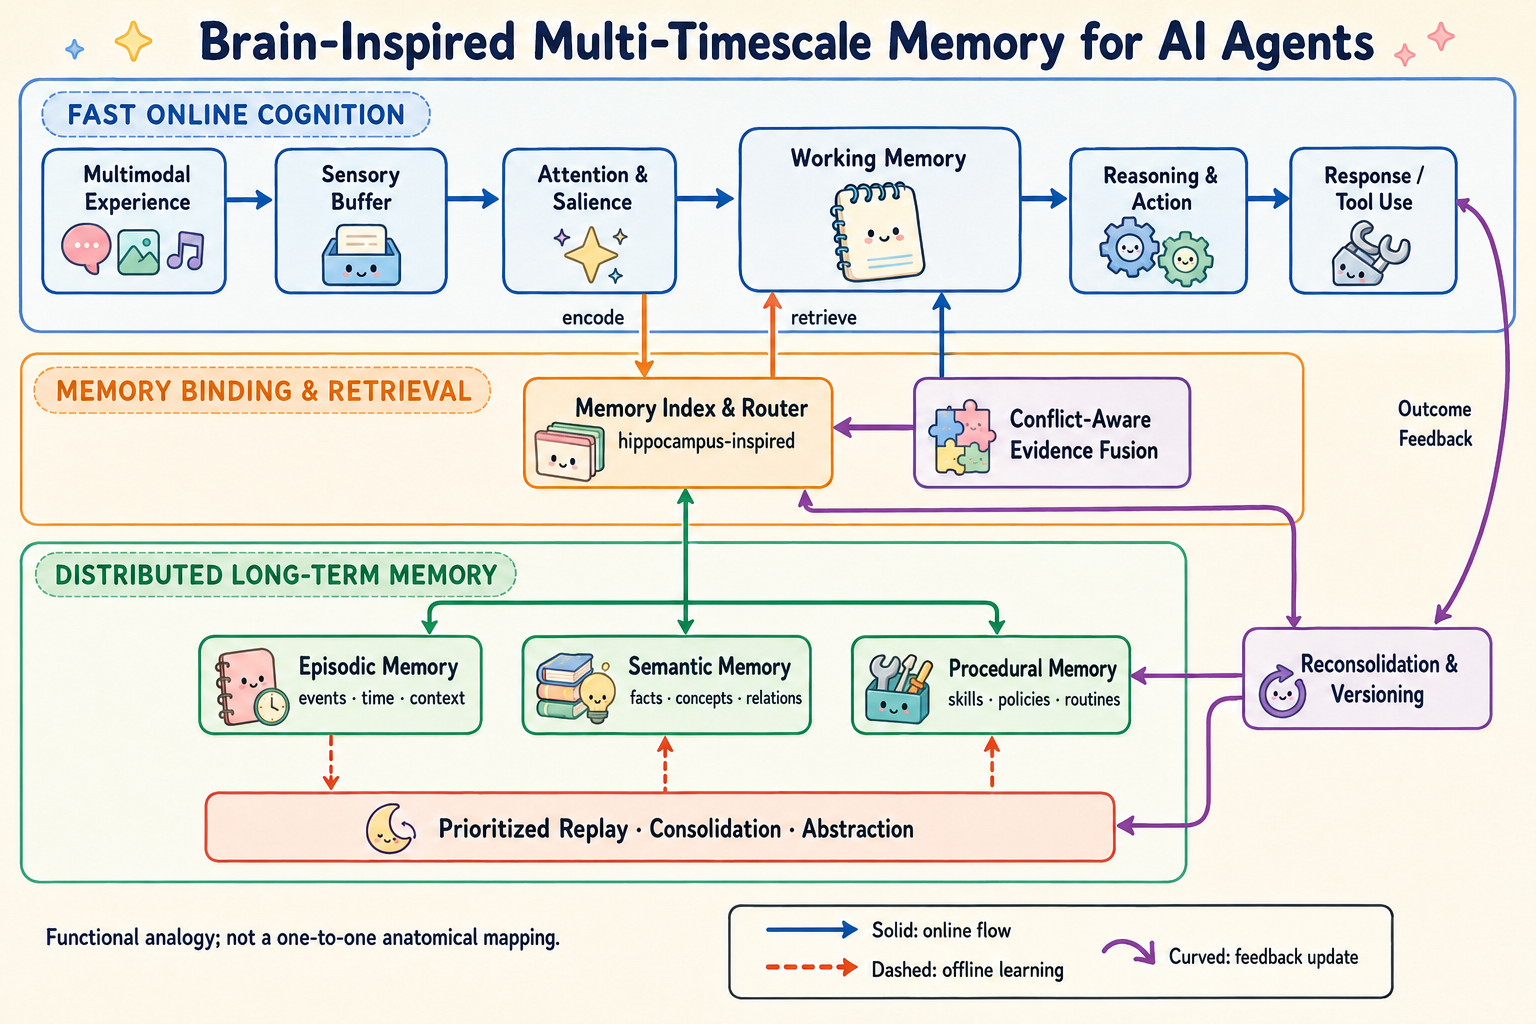
\includegraphics[width=\textwidth]{figures/framework.png}
\caption{The supplied multi-timescale framework, reproduced unchanged.
Brain-region labels express functional inspiration, not anatomical equivalence.
The paper formalizes encoding, typed memory, evidence fusion, and versioned
reconsolidation; its initial evaluation covers conversational text, not every
multimodal or action interface shown.}
\label{fig:framework}
\end{figure}

\subsection{State and functional organization}
At interaction step $t$, the persistent state is
\begin{equation}
 M_t=(\E_t,\Sema_t,\Proc_t,\Graph_t,\Queue_t),
 \qquad W_t=\operatorname{Assemble}(q_t,M_t;B),
\end{equation}
where $W_t$ is the working context and $B$ is its memory-token budget.
$\Queue_t$ holds pending consolidation and repair jobs. The three memory
types are logical roles; they need not require three different databases.
The language model, embedding model, and verifier are frozen in the proposed
initial evaluation. Adaptation changes external memory, not model weights.
The working context is the information currently exposed to the reader; the
hippocampus-inspired index is a binding mechanism, not a model of hippocampal
anatomy. Retrieval-related reconsolidation provides a further functional
motivation, but its biological evidence includes specific experimental
settings such as fear-memory studies in rats~\citep{brain_reconsolidation}.
That evidence does not establish the validity of our computational design.

\paragraph{Episodic memory: what happened.}
Each episode $e=(\mathrm{id},x,a,t_o,t_e,\sigma)$ stores its observed content
$x$, speaker or tool $a$, observation time $t_o$, optional event time $t_e$, and
source offsets $\sigma$. Records are append-only during normal operation.
A correction is a new observation, not an erasure of the original event.
An assistant statement is labeled as such and is not treated as an independently
verified fact. In the conversational setting, the source establishes what a
participant reported, not necessarily objective truth about the world.

\paragraph{Semantic memory: what the evidence supports.}
A semantic record contains a proposition, entity and relation keys, temporal
scope, source-span dependencies, a version, and a status in
\{active, disputed, superseded, stale\}. A derived relation may depend on
several episodes. Event time, observation time, and validity interval are
separate fields; an absent interval remains unknown. A provenance pointer
records the origin of a claim but does not by itself prove entailment.

\paragraph{Procedural memory: how to use experience.}
A procedure contains an applicability condition, ordered retrieval or action
steps, an expected observable check, supporting use traces, and a version.
For example, ``resolve a demonstrative by locating the earlier recommendation
between the same participants'' is a retrieval procedure; ``the book is
\emph{Becoming Nicole}'' is not. Learned procedures are candidates until
validated on distinct development episodes. Every stored procedure is marked
as either a fixed seed rule or an experience-derived rule. This prevents
hand-written instructions from being reported as learned skills.

\begin{table}[t]
\centering\small
\begin{tabularx}{\textwidth}{@{}lXX@{}}
\toprule
Timescale & Operation & Committed state change \\
\midrule
Fast encoding & Buffer, preserve source, extract cues & Append episode and index; queue abstraction \\
Query-time binding & Route, retrieve, fuse, respond & Log evidence use; flag supported conflicts \\
Slow integration & Replay, abstract, validate, revise & Version affected semantic/procedural records \\
\bottomrule
\end{tabularx}
\caption{Functional interpretation of the supplied framework. Slow integration
is a scheduling choice, not a simulation of biological sleep.}
\label{tab:timescales}
\end{table}

\subsection{Fast encoding and typed evidence retrieval}
The sensory buffer groups incoming turns into source-preserving episodes.
Salience controls indexing and replay priority, not irreversible deletion:
low-salience observations remain available as episodes. Named entities,
relations, explicit dates, corrections, and unresolved references are indexed.
New episodes become retrievable before consolidation finishes. At a session
boundary or a fixed buffer threshold, the agent queues related episodes for
semantic integration; it does not regenerate its entire memory after each turn.

A bounded router maps a query to entity/relation cues, a requested time scope,
and optional procedure preconditions. It retrieves candidates from $\E_t$
and $\Sema_t$ using the same sparse--dense rank fusion, while $\Proc_t$ is
searched for applicable strategies. The top matching procedure may specify
one additional evidence lookup, such as searching for an earlier recommendation.
Unmatched preconditions cause the procedure to be skipped, not forced onto
the query. This design makes procedure use observable and limits recursive
retrieval cost.

Candidate semantic claims are expanded to their recorded episode dependencies.
The resulting unit of selection is an \emph{evidence bundle}: a claim together
with the source spans needed to interpret it. Bundles share deduplicated
sources. They are greedily admitted by query relevance per newly added token
under $B$, subject to their temporal applicability. A required evidence bundle
that does not fit is skipped intact rather than silently losing a dependency.
The memory budget includes procedure text and metadata exposed to the reader.
This is a bounded heuristic, not an optimal retrieval algorithm.

\subsection{Conflict-aware evidence fusion}
Fusion produces a compact ledger of supported claims, their scopes, and
unresolved alternatives before the reader answers. It distinguishes three
cases. Complementary records can be joined through a supported relation or
coreference link. A later explicit correction to the same scoped attribute
can supersede its previous current value. Incompatible records without a
justified precedence relation remain disputed. A later timestamp alone does
not establish that an unrelated event replaces an earlier one.

For a current-state query, superseded values are not presented as current.
For a historical query, the earlier value remains usable within its original
scope. A verifier checks the proposed claim against the actual cited spans;
when the evidence is ambiguous, the ledger preserves that ambiguity and the
reader can abstain. Model verification is fallible and is not a correctness
guarantee. In particular, knowing a title from the LLM's parameters is not
evidence that a specific participant read that title.

The output is paired with a use trace
\begin{equation}
 u_t=(q_t,\mathrm{versions}(D_t),\pi_t,\widehat y_t,o_t),
\end{equation}
where $D_t$ is the used evidence set, $\pi_t$ is the applied procedure, and
$o_t$ is any available external outcome. An absent outcome is recorded as
unknown. The trace is a dependency record, not a chain-of-thought transcript.

\subsection{Evidence-bound reconsolidation}
\label{sec:reconsolidation}
The dependency graph contains typed \texttt{derived-from}, \texttt{used-by},
and \texttt{supersedes} edges. The first two point from supporting records to
their dependents. A supported correction identifies a seed set $C_t$ of
directly contradicted or invalidated records. The repair set is
\begin{equation}
 A_t=C_t\cup\operatorname{Desc}_{\{\mathrm{derived},\mathrm{used}\}}
       (C_t;\Graph_t).
 \label{eq:closure}
\end{equation}
Only dependencies on the invalidated scope or exact version propagate the
flag. A procedure that merely retrieved a corrected fact is not automatically
false; its previous use trace becomes outdated, while the procedure itself is
revalidated only if its applicability or validation depends on that fact.

Immediately after identifying a correction, affected derived records are
marked stale. They cannot be served as active support while repair waits in
the background queue. The original episodes remain retrievable, including
the new correction. This separates fast invalidation from expensive rewriting:
asynchronous consolidation must not create a window in which already-known
stale claims are still treated as valid.

Replay schedules explicit contradictions first, then unsupported-use reports,
then ordinary abstraction jobs. Within a class it prioritizes the number of
affected active dependents, breaking ties by waiting time. This is an explicit
scheduler, not a learned priority policy. Each job reads the relevant source
episodes and reconstructs semantic candidates with their dependencies.
Successful, externally checked development traces may also yield a generalized
procedure; one correct answer is insufficient evidence of transfer.

A revision commits only after source-span checks, temporal-scope checks, and
dependency validation. All replacements in a repair transaction receive new
versions, and the previous versions remain auditable. If the source snapshot
changes before commit, the job is retried against the new snapshot. If a
verification check fails or the computation budget is exhausted, the disputed
or stale state remains explicit; the system does not restore an unsupported
claim simply to finish the update. Unrelated active records are not rewritten.
Missing or incorrect dependency edges can nevertheless make a repair incomplete.

\begin{algorithm}[t]
\caption{Multi-timescale operation with evidence-bound reconsolidation}
\label{alg:mtm}
\begin{algorithmic}[1]
\Require Stream observations $x_t$, optional queries $q_t$, memory $M_t$
\State Append source-labeled $x_t$ to $\E$; update cues and pending jobs
\State Identify explicit scoped corrections; mark their dependent records stale
\If{a query $q_t$ is present}
  \State Route to episodic/semantic candidates and an applicable procedure
  \State Expand dependencies; pack complete evidence bundles within $B$
  \State Fuse by source support and temporal scope; answer or abstain
  \State Record the used versions, procedure, output, and observed outcome
  \State Queue evidence-supported conflicts; never use benchmark labels
\EndIf
\If{a consolidation boundary is reached}
  \State Select jobs by conflict class, dependency impact, and waiting time
  \State Replay their source episodes; propose abstractions or scoped repairs
  \State Validate support and dependencies; commit versioned replacements
\EndIf
\end{algorithmic}
\end{algorithm}

\paragraph{What the mechanism does and does not establish.}
Equation~\ref{eq:closure} guarantees only that the \emph{recorded} dependency
closure is considered when the algorithm is implemented correctly. It does
not guarantee that all real semantic dependencies were extracted. Likewise,
versioning supports traceability, not truth. The research hypothesis is that
making these dependencies explicit improves revision locality and future
answers enough to justify the additional retrieval and maintenance cost.

\FloatBarrier
\section{A Source-Grounded LoCoMo Example}
\label{sec:example}
We checked the supplied example against conversation \texttt{conv-26} in the
LoCoMo release. Turn \texttt{D7:11}, dated July 12, 2023, contains Caroline's
recommendation of \emph{Becoming Nicole}. Turn \texttt{D17:10}, dated October
13, 2023, contains Melanie's report of reading a previously recommended book.
The dataset's question asks which book Melanie read following Caroline's
suggestion; its reference answer is \emph{Becoming Nicole}, with both turn
IDs listed as evidence. The official evaluator identifies category 1 as
multi-hop; we retain this released label.

\begin{figure}[!ht]
\centering
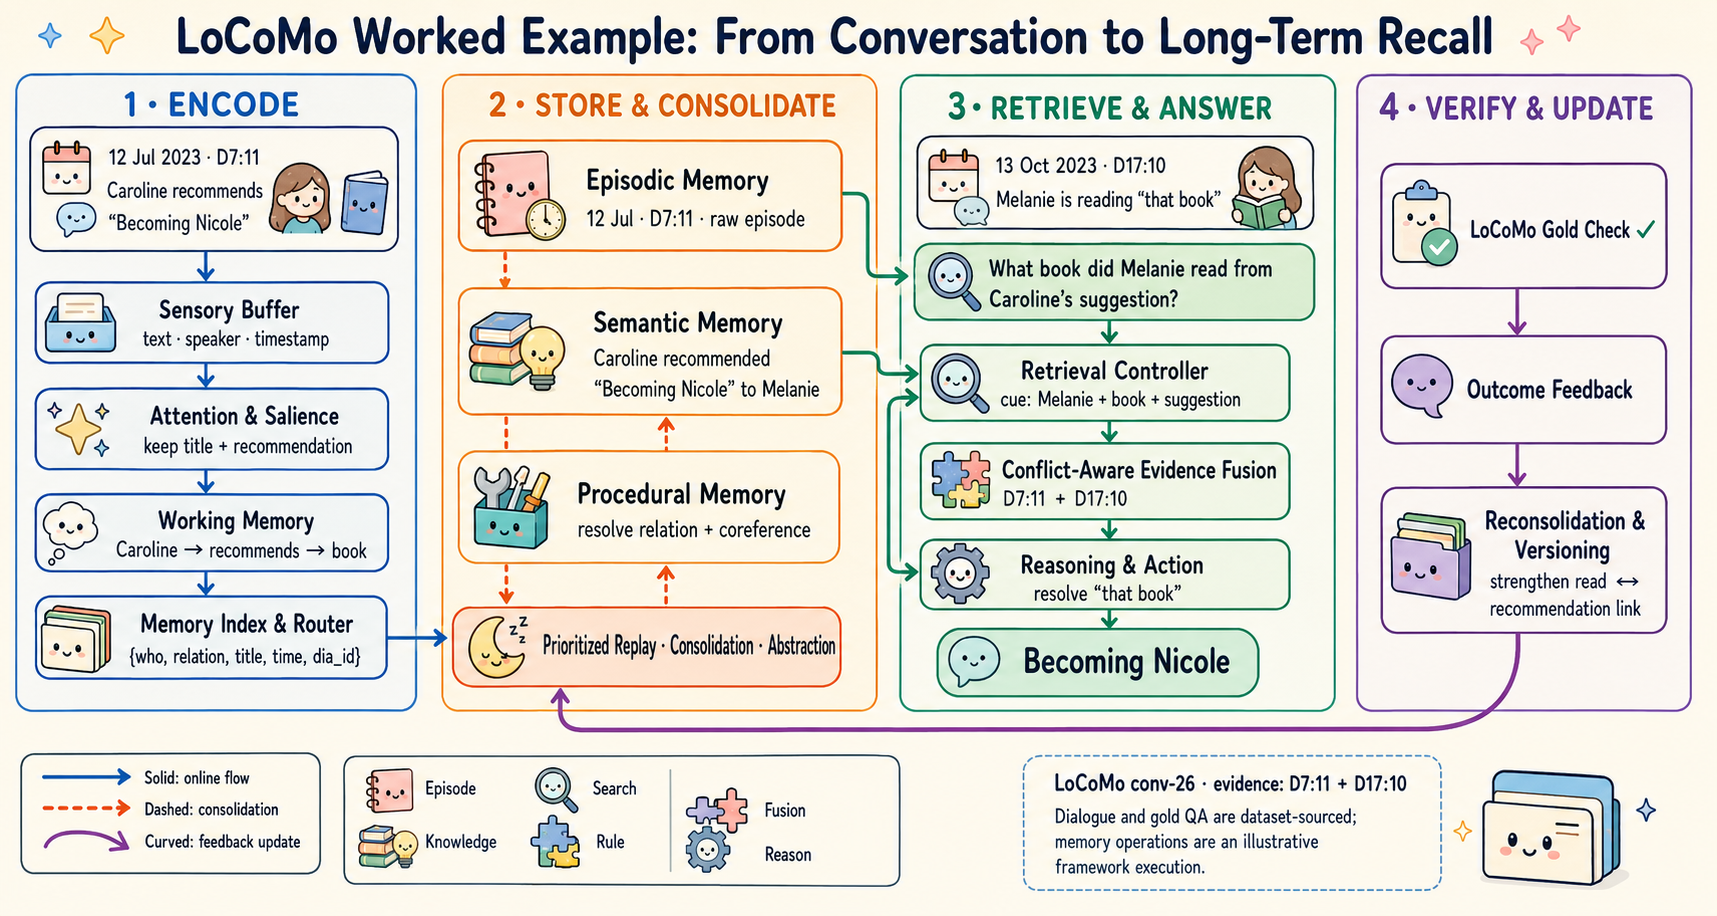
\includegraphics[width=\textwidth]{figures/framework_locomo_example.png}
\caption{The supplied LoCoMo example, reproduced unchanged. The two turns and
reference answer were checked against \texttt{conv-26}; memory operations are
illustrative, not execution logs. The ``Gold Check'' branch is
\emph{evaluator-only}: neither gold answers nor grading feedback may enter
test-time reconsolidation, despite the feedback arrow in the illustration.}
\label{fig:locomo-example}
\end{figure}

The episodic store preserves both utterances and their dates. Semantic
consolidation can propose a recommendation relation grounded in the first
turn and a later reading relation whose book argument is initially unresolved.
The router identifies the shared participants and recommendation relation,
then retrieves the earlier episode. An applicable procedure instructs the
agent to check this relation before resolving the demonstrative. Fusion can
then propose the title with both source spans attached. If other compatible
recommendations remain, it must preserve uncertainty rather than choose a
title solely from semantic similarity.

This example reveals three separable failure points: losing the original
recommendation during encoding, retrieving the later turn without its
antecedent, or asserting an unsupported cross-session link. They require
different repairs. Repeating the same answer is not a repair signal, and
retrieving a source ID is not proof that its answer-bearing text was available.
Figures~\ref{fig:framework} and~\ref{fig:locomo-example} show the corresponding
architecture and worked example, not measured model performance.

\paragraph{Separating evaluation from adaptation.}
The ``LoCoMo Gold Check'' in the supplied illustration belongs strictly to
the evaluator. Its result must not be fed into the test-time memory update
loop. Memory is built from the native history in chronological order, allowing
later observations to trigger reconsolidation during ingestion. Each question
then starts from an isolated copy of that history-only snapshot; query-induced
changes cannot help later questions. This tests update-aware memory without
exposing held-out answers or inventing an additional feedback benchmark.

\FloatBarrier
\section{Experimental Design}
\label{sec:experiments}
We use only LoCoMo and LongMemEval, with three complementary analyses below.
All measurements are pending. Table~\ref{tab:benchmarks} fixes the evaluation
scope; no synthetic update benchmark or additional test questions are added.
Native images/audio and general tool-use competence are outside this scope.

\begin{table}[!ht]
\centering\small
\begin{tabularx}{\textwidth}{@{}lXX@{}}
\toprule
Benchmark & Evaluation set & Primary score \\
\midrule
LoCoMo & 10 conversations; 1,540 questions in categories 1--4 & Official category-specific F1, averaged over questions \\
LongMemEval & Cleaned S release; 500 questions & Accuracy under the official question-type and abstention rubrics \\
\bottomrule
\end{tabularx}
\caption{Two-benchmark protocol \citep{mrw_locomo,mrw_longmemeval}.
LoCoMo category 5 is excluded explicitly; LongMemEval uses cleaned S, not M,
oracle, or V2. Scores are reported separately, never averaged across benchmarks.}
\label{tab:benchmarks}
\end{table}

\paragraph{Shared protocol.}
Ingest full conversations chronologically, preserving speakers, dates, and
provided text captions. Exclude test questions, answers, evidence labels,
answer-session IDs, and answer-bearing-turn flags from indexing and replay;
do not ingest released precomputed summaries. Use the supplied question date
at inference and reset query-induced changes between questions. Freeze model
versions, decoding, prompts, dataset hashes, and the judge configuration
before evaluation. Procedures are induced and validated only on independent
development dialogues, then frozen before benchmark ingestion.

\subsection{Accuracy and total cost}
Compare \method{} with raw-history hybrid RAG, LightMem, HippoRAG~2, and
Hindsight. Use their upstream implementations with pinned revisions, not
prompt-only imitations. Match the reader, embedding and memory-writing models
where supported, preprocessing, and a 4K-token retrieved-memory budget,
including exposed procedure text and metadata. Disclose unsupported controls
instead of silently changing a baseline.

Report each benchmark's primary score, online p50/p95 latency, and total
model input/output tokens. Separate history construction and replay from
query-time routing, retrieval, verification, and answering. Amortize each
history's construction over its evaluated questions; count procedure
development once and disclose it separately. Include active and archival
storage, and keep evaluator-only grading cost separate. The result is one
accuracy--cost table, not a large model-by-budget grid.

\subsection{Contribution of the core mechanisms}
At the same 4K budget, compare the full system with three removals:
\emph{no procedural reuse}, using the fixed default router;
\emph{no conflict-aware fusion}, passing the same retrieved bundles directly
to the reader; and \emph{no evidence-bound reconsolidation}, retaining new
episodes and periodic consolidation but disabling dependency-local
invalidation and repair. Keep source access, other prompts, session-boundary
schedules, and compute ceilings fixed; report realized costs. Use three
matched seeds for full and ablated systems and report the mean and variation.

If claiming learned procedures, also compare against a same-budget fixed seed
library. An advantage over no procedures alone demonstrates useful procedure
access, not learning. These comparisons form one compact ablation table.

\subsection{Relational, temporal, and update-aware reasoning}
Reuse the same runs and official questions: inspect LoCoMo's multi-hop and
temporal categories, and LongMemEval's multi-session, temporal-reasoning,
knowledge-update, and abstention subsets. The abstention subset is identified
by the release's question-ID suffix, not an invented question type.
Compare full and ablated scores to test whether binding and repair help the
capabilities they target. Add evidence recall using LoCoMo's annotated turns
and LongMemEval's answer sessions where available; score the source text
actually exposed to the reader, not merely retrieved IDs. Partial sessions
count only when an annotated answer-bearing turn is present. These labels
remain evaluator-only. Summarize category effects in one figure.

Report paired 95\% bootstrap intervals grouped by conversation or independent
history, with seeds matched across ablations. LoCoMo has only ten independent
conversations, limiting uncertainty estimates. Use every item in the declared
sets; retain failed calls in the denominator and report their count and retry
policy. Native knowledge-update questions test revision during history
ingestion; they do not by themselves establish post-answer lifelong learning
or complete dependency-repair correctness.

\section{Limitations and Research Risks}
The framework is presently an algorithmic proposal, not an empirically
validated system. Its hardest component is reliable dependency extraction:
an incorrect link can create a false abstraction, while a missing link can
prevent the necessary repair. Source-grounded verification can still fail,
and repeated model agreement is not independent confirmation. Temporal
interpretation and conflicting user reports may remain unresolved.

Procedural memory also introduces an attribution problem. A useful fixed
retrieval instruction is not evidence that the system learned a reusable
strategy from experience. The specified seed-rule control and held-out
procedure validation are therefore necessary. QA success would establish
conversational utility, not general action learning or multimodal cognition.

Typed stores, provenance, feedback, and sleep-time updates all have substantial
precedent. The proposed coupling may offer little beyond a strong existing
system, or its extra verification may outweigh the accuracy benefit. Negative
results would restrict the framework's useful operating conditions; they
should not be obscured by changing budgets or omitting background costs.
Finally, append-only episodic storage raises privacy and storage concerns.
Deployment needs authorized deletion and dependent-record removal; research
versioning must not be presented as a reason to retain personal data forever.

\section{Conclusion}
We propose a brain-inspired memory framework in which episodes provide
evidence, semantic memory captures scoped knowledge, and procedural memory
guides evidence use. Its central idea is to reuse the dependencies created
during abstraction and retrieval for targeted, versioned reconsolidation.
The verified LoCoMo case motivates relational binding; evaluation on LoCoMo
and LongMemEval separates accuracy and cost, component effects, and
relational, temporal, and update-aware reasoning.
Whether this coupling improves long-term agent memory at an acceptable cost
is the empirical question the proposed experiments must answer.

\section*{AI Use Statement}
Generative AI assisted with literature inspection, framework formalization,
experimental-design refinement, manuscript drafting, and LaTeX preparation.
No benchmark measurements were generated or inferred in preparing this draft.
Author review of the scientific claims, references, and final disclosure is
required before submission. The origin and editing history of supplied
illustrations must also be confirmed by the authors for the final disclosure.

\section*{Reproducibility Statement}
The algorithm, budget rules, and evaluation boundaries are specified in
Sections~\ref{sec:method}--\ref{sec:experiments}, with both supplied conceptual
figures in the main text and implementation contracts in the appendix. An executable end-to-end
implementation, run manifests, and benchmark outputs are still required.
The worked example is a dataset check, not a reproduced system experiment.

\bibliographystyle{iclr2027_conference}
\bibliography{related_work_20260903,references_extra}

\appendix
\clearpage
\section{Implementation and Evaluation Contracts}
\label{app:contracts}
\paragraph{A minimal implementation.}
Represent episodic records, semantic claims, procedures, use traces, and
version edges in a local transactional store. Build a shared sparse--dense
index with type filters; rank fusion must be identical across ablations.
The initial router is a frozen model call returning entity keys, relation
keys, temporal scope, and at most one applicable procedure. Fix a maximum
of two retrieval rounds: initial retrieval and one procedure-requested lookup.
Use a source verifier that returns supported, contradicted, or unresolved,
with exact source offsets. Treat parser failure as a system failure, not
silently as abstention or an incorrect answer.

\paragraph{Record and transaction invariants.}
Every active semantic record has at least one resolvable episode-span
dependency. Every derived edge identifies the source version and scope.
A use trace stores the exact versions read. Commit a repair only against the
source snapshot from which it was constructed. Mark known-stale descendants
unavailable before scheduling a rebuild. Historical applicability and
current applicability are checked separately. A failed repair never silently
reactivates a stale claim. These invariants check software behavior; they do
not validate the semantic correctness of extracted claims.

\paragraph{Procedure induction.}
Start with a small declared seed library shared by full and control systems.
Use independently generated development dialogues, split by source-template
family before generating paraphrases, with no benchmark passages, questions,
or answers. Fix the generation templates and procedure-selection criteria
before benchmark runs and record the full development-generation cost.
Generate candidate procedures only from source-grounded development use
traces or externally verified training interactions. Abstract entity names
and answer strings out of the procedure. Validate its preconditions and
observable check on distinct held-out development episodes, all separated
from benchmark histories. Store the validation trace IDs and retire a
procedure when its supporting conditions are invalidated. The benchmark
test set cannot supply demonstrations, correction labels, or induction
targets. No claim of learned procedural memory is warranted until this
pipeline and its fixed-rule control have been evaluated.

\paragraph{Replay and scheduling.}
Use session boundaries for ordinary consolidation and a fixed compute cap
per boundary for every compared method. Explicit scoped contradictions
create immediate invalidation jobs. Queue ordering is lexicographic:
conflict class, number of active dependents, then elapsed queue time.
Record queue length, actual jobs completed, and source tokens examined.
When support cannot be recovered within the budget, leave the item disputed
and record the deferred work. Report any global graph scan separately from
dependency-local repair time; a local update set does not prove local search
cost.

\paragraph{History-only adaptation and isolated QA.}
Construct memory from chronologically revealed benchmark conversations;
replay may use only observations already seen. Use identical boundary budgets
for full and no-reconsolidation variants. Clone the final history-only state
for each official question, preserve its question date, and discard all
query-induced changes after answering. Keep gold answers, annotated source
IDs, and answer-bearing flags in a separate evaluator. LongMemEval abstention
uses the official question-ID mask; it is not a seventh question type.
No generated corrections, additional test questions, or separate longitudinal
benchmark enter the reported scores.

\paragraph{Required evidence before submission.}
The new framework still requires an integrated implementation; validated
procedure induction; official-baseline runs; full LoCoMo and LongMemEval
results; and the three matched comparisons in Section~\ref{sec:experiments}.
A runnable module, a conceptual figure, or a successful unit test alone does
not establish any of these empirical claims. No result table is populated
in this draft because these measurements have not been supplied.

\end{document}
